\documentclass{ximera}
 
 
% \input{../preamble.tex}
 
      
\title{MAT 211 (Calculus I) Activity}
      
\begin{document}
      
\begin{abstract}
      
Some sample questions that can be related to MAT 211, Calculus I.
.
      
\end{abstract}
      
\maketitle
      
      
\begin{question}      
Consider the function $f(x)=\begin{cases}x+1 & x<3 \\ -\frac{x^2}{3}+8 & x\geq 3\end{cases}$.

\begin{onlineOnly}
$$\graph[xmin=-10,xmax=10]{x+1\left\{x<3\right\}, \frac{x^2}{3}-8\left\{x\ge 3\right\}}$$
\end{onlineOnly}


\begin{itemize}
\item The limit of $f$ as $x$ approaches 3 from the left is $\displaystyle\lim_{x\to 3^-}=\answer[]{4}$.
\item The limit of $f$ as $x$ approaches 3 from the right is $\displaystyle\lim_{x\to 3^+}=\answer[]{5}$.
\item The actual value of $f$ when $x=3$ is $f(3)=\answer[]{5}$.
\item From this what can we conclude:
\begin{multipleChoice}
\choice{$f(x)$ is continuous at $x=3$.}
\choice[correct]{$f(x)$ is not continuous at $x=3$.}
\choice{We do not have enough information to determine the continuity of $f(x)$ at $x=3$.}
\end{multipleChoice}

\end{itemize}


\end{question}


\begin{question}
Consider the function $f(x)=\sqrt{x}$.  

\begin{onlineOnly}
$$\graph[xmin=-1,xmax=10, panel]{f(x)=x^{.5},m=(f(a+h)-f(a))/h,  y=m(x-a)+f(a), a=0, h=1}$$
\end{onlineOnly}
(Use the sliders for $a$ and $h$ to find the point where you wish to estimate the derivative and the accuracy of that estimate.  Note that you may change $f(x)$ to do the same estimations with other functions.  A fully functional version of this graph may be found here: \url{https://www.desmos.com/calculator/1tkd8mob7k}.)

Recall that the difference quotient for any function $f$ when $x=a$ and given some real number $h$ is $$\frac{f(a+h)-f(a)}{h}$$

\begin{enumerate}
\item The difference quotient for $f$ when $x=1$ and $h=0.5$ is approximately $\answer[ ]{0.4495}$ (Round to four decimal places). 
\item The difference quotient for $f$ when $x=3$ and $h=0.1$ is approximately $\answer[ ]{0.2863}$ (Round to four decimal places).\\ \\
\item We will now compute the limit definition of the derivative of $ f'(x):={\displaystyle \lim_{h\to 0}} \frac{f(x+h)-f(x)}{h}$.

\begin{eqnarray*}
f'(x)&=&{\displaystyle \lim_{h\to 0}} \frac{f(x+h)-f(x)}{h}\\
&=& \displaystyle \lim_{h\to 0}\frac{(\answer{\sqrt{x+h}})-(\answer{\sqrt{x}})}{h}\\
&&\text{We must remove the zero divisor. }\\ && \text{A familiar way to do this is through conjugation:}\\
&=& \displaystyle \lim_{h\to 0}\frac{(\answer{\sqrt{x+h}})-(\answer{\sqrt{x}})}{h}\cdot \frac{\answer{\sqrt{x+h}}+\answer{\sqrt{x}}}{\answer{\sqrt{x+h}}+\answer{\sqrt{x}}}\\
&&\text{So by difference of squares:}\\
&=& \displaystyle \lim_{h\to 0}\frac{(\answer{x+h})-(\answer{x})}{h\left(\answer{\sqrt{x+h}+\sqrt{x}}\right)}\\
&=& \displaystyle \lim_{h\to 0}\frac{\answer{h}}{h\left(\answer{\sqrt{x+h}+\sqrt{x}}\right)}\\
&&\text{Then by cancelling $h$:}\\
&=& \displaystyle \lim_{h\to 0}\frac{\answer{1}}{\left(\answer{\sqrt{x+h}+\sqrt{x}}\right)}\\
&&\text{Now we can evaluate $h=0$ without dividing by zero!}\\
&=&\frac{\answer{1}}{\answer{\sqrt{x}}+\answer{\sqrt{x}}}\\
&=& \answer{\frac{1}{2\sqrt{x}}}
\end{eqnarray*}


\end{enumerate}

Note that you may adjust the function $f(x)$ in the above graph to be any function you like, and examine the appropriate secant lines and difference quotients at your leisure!


\end{question}


\begin{question}

Suppose you are standing on top of a 50 foot ladder that is leaned against a wall such that the top is 40 feet off the ground.  Suddenly a very inconsiderate friend thinks its funny to yank out the ladder from under you!  Suppose that they yank the ladder out at a speed of 2 feet per second.  How fast will you start dropping?

\begin{explanation}

Let's let $y$ denote your height off the ground and $x$ the distance from the base of the ladder to the wall.  The 50 foot ladder then acts as the hypotenuse of some right triangle.  So when your height is $y=40$ feet, we may use Pythagorean's theorem to see that $x=\answer{30}$ feet.

The change in $x$ over time, represented by $\frac{dx}{dt}$ is positive, since the distance from the wall is increasing, and the magnitude of this change is 2 feet/sec.  Thus $\frac{dx}{dt}=\answer{2}$ feet/sec.

Similarly, $\frac{dy}{dt}$ which represents your change in height, ought to be:

\begin{multipleChoice}
\choice{positive}
\choice[correct]{negative}
\choice{zero}
\end{multipleChoice}

\ldots which make sense as you are falling.  We can put this all together in the following picture:

\begin{image}
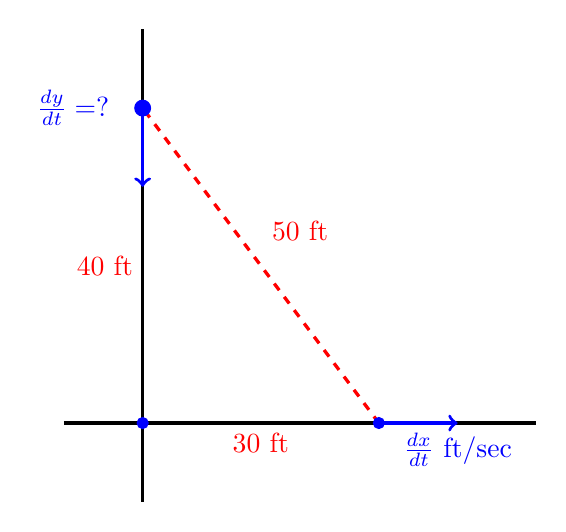
\begin{tikzpicture}
\draw[very thick] (-1,0) -- (5,0);
\draw[very thick] (0,-1) -- (0,5);
\draw[->,blue, very thick] (0,4) -- (0,3);
\draw[->,blue, very thick] (3,0) -- (4,0);
\draw[dashed,red, very thick] (3,0) -- (0,4);

%\node[blue,rotate=90,right] at (.5,3) {\scalebox{-2} \Bicycle};
\node[blue,left] at (-.3,4) {$\frac{dy}{dt}=?$};
\node[red,left] at (0,2) {$40$ ft};
\node[red,below] at (1.5,0) {$30$ ft};
\node[blue,below] at (4,0) {$\frac{dx}{dt}$ ft/sec};
\node[red,above] at (2,2.2) {$50$ ft};
%\node[blue,right,above] at (3.5,0) {\scalebox{-2}[2] \Bicycle};

\draw [blue, fill] (0,0) circle [radius=.07];
\draw [blue, fill] (3,0) circle [radius=.07];
\draw [blue, fill] (0,4)circle [radius=.1];


\end{tikzpicture}
\end{image}

To actually find $\frac{dy}{dt}$, we revisit our old friend implict differentiation.  Consider that for any possible values for $x$ and $y$, it must be that:

\begin{eqnarray*}
x^2+ y^2 &=& 50^2\\
&&\text{Differentiating both sides with respect to $t$ gives us:}\\
\answer{2x}\frac{dx}{dt}+\answer{2y}\frac{dy}{dt}&=& 0\\
\text{Evaluating this expression for known values gives us:}\\
\answer{120}+\answer{80}\frac{dy}{dt}&=& 0\\
\frac{dy}{dt}&=& \answer{-1.5}\ \text{feet/sec}
\end{eqnarray*}

That's not good!  But it get's worse.  What about when you're 5 feet off the ground?  We see that $x=\answer{\sqrt{2500-25}}$ feet, and thus $\frac{dy}{dt}=\answer{-\sqrt{2500-25}/5}$ or approximately $\approx \answer{-9.9499}$ (round to 4 decimal places) feet/sec!


\end{explanation}

\end{question}



\begin{question}
Consider $f(x)=x^2-3x$

\begin{onlineOnly}
$$\graph[xmin=-1, xmax=7, panel]{F=x^2-3x, F<y<0\left\{0<x<3\right\},0<y<F\left\{3<x<6\right\}}$$
\end{onlineOnly}
(The above graph shows the curve $y=f(x)$. Go  \url{https://www.desmos.com/calculator/o2jdhyeocq} for a version of this graph that visualizes and computes  the Riemann sums.  Use $a, b$ to adjust your end points, $n$ for the number of rectangles, and $c$ for the method (left, right or midpoint).  One may also adjust $f(x)$ to do the same for other graphs.)


\begin{enumerate}
\item Use $n=2$ intervals and the left hand sum to estimate $\displaystyle\int_0^6 x^2-3x\ dx$. \\ \\
\begin{explanation}
Notice that if $n=2$, then the length of each interval is $\answer{3}$.  Then taking the left endpoint of each interval, the sum of the signed area of our rectangles (in ascending order of $x$) is: $$\answer{3}(f(\answer{0})+f(\answer{3}))=\answer{3}(\answer{0}+\answer{0})=\answer{0}.$$
\end{explanation}




\item Use $n=3$ intervals and the right hand sum to estimate $\displaystyle\int_0^6 x^2-3x\ dx$. \\ \\
\begin{explanation}
Notice that if $n=3$, then the length of each interval is $\answer{2}$.  Then taking the right endpoint of each interval, the sum of the signed area of our rectangles (in ascending order of $x$) is: $$\answer{2}(f(\answer{2})+f(\answer{4})+f(\answer{6}))=\answer{2}(\answer{-2}+\answer{4}+\answer{18})=\answer{40}.$$

\item Following the same arguments about, if $n=6$, the left hand sum will be $\answer{10}$ and the right hand sum will be $\answer{28}$.

\end{explanation}
 Note that you can use the sliders in the above graph to do these computations!  Let $a,b$ be your endpoints, $n$ the number of rectangles and let $c=0$ for left hand sums, $c=0.5$ for midpoints, and $c=1$ for right hand sums.


\item Compute $\displaystyle\int_0^6 x^2-3x\ dx$. 
\begin{explanation}
So by the Fundamental Theorem of Calculus:

\begin{align*}
displaystyle\int_0^6 x^2-3x\ dx&\ =\ \answer{x^3/3-3x^2/2}\Big|_0^6\\
&\ =\ \answer{18}-\answer{0}\\
&\ =\ \answer{18}.
\end{align*}



\end{explanation}



\end{enumerate}


\end{question}








\end{document}
